% Chapter Template

\chapter{Problem Specification} % Main chapter title

\label{Chapter4} % Change X to a consecutive number; for referencing this chapter elsewhere, use \ref{ChapterX}

\lhead{Chapter 4. \emph{Problem Specification}} % Change X to a consecutive
% number; this is for the header on each page - perhaps a shortened title

%----------------------------------------------------------------------------------------
%	SECTION 1
%----------------------------------------------------------------------------------------

\section{Problem Specification}
\label{problem}

The DPF Workbench already includes support for model transformations inn form
of code generation. However, the environment does not include support for
transforming a model between different modeling languages. One of DPF's
strengths is that it is possible to formally define a Domain Specific Modeling
Language by defining multiple levels of meta-models. The main goal of this
thesis is to extend the DPF Workbench with exogenous model to model
transformations. This leads to the main question for this thesis.
 
\begin{itemize}
  
  \item Can we include tool support for model to model transformations for the
  DPF Workbench that translates a model specified over a modeling hierarchy to a
  model specified over another modeling hierarchy?

\end{itemize}

The solution to this is not written in stone, and there are several approaches
to how we can solve this specific problem. The tool requires some manual
implementation but there are several existing approaches available that provides model
transformations as we mentioned in section~\ref{tooling}. DPF specifications are
basically graphs, more specific, they are directed graphs. This means that a
DPF specification consist of a set of nodes, arrows and two functions
that specifies source and target node of the edges. This makes a graph based
approach to model transformations convenient, but we should also consider other
approaches to model transformations.

\begin{itemize}
  
  \item Can we integrate an existing model transformation environment with an
  editing tool for the Diagram Predicate Framework Workbench?

\end{itemize}

We want to introduce the DPF Workbench with tool support that includes model
transformations. This has already been partially introduced to the workbench
environment in Anders Sandven\cite{Sandven_thesis}'s master thesis. In his
thesis he describe how he integrated a M2T transformation environment to the DPF
Workbench. He integrated a model transformation environment, Xpand\cite{Xpand}
that provides a template based approach to Model2Text transformation. For this
thesis however, we want to verify that we can successfully introduce a model
transformation environment that supports translation between different DSML's.
But first we have to find an applicable environment that can be integrated with
the DPF Workbench. In section~\ref{tools} we will explore three different
model transformation tools that supports both exogenous and endogenous model
transformations. One aspect of model transformations that is required to
translate specifications in DPF is a set of transformation rules that describes
how a target model is produced. This leads to a problem for the DPF, because a
transformation rule requires modeling elements from some abstract syntax to
specify a structural pattern that is used to locate matches in a source model. 

\begin{itemize}  

  \item How can we include the abstract syntax of a modeling language that is
  specified by a corresponding linguistic meta-model and a corresponding 
  ontological meta-model for a single transformation rule.

\end{itemize}

In 2007 Ralf Gitzel, Ingo Ott and Martin Schader published a paper where they
amongst other subjects discuss the difference between Linguistic and
Ontological meta-modeling. They provide a definition between the two, 
\textit{``Linguistic metamodeling uses a metamodel to describe a language syntax
without a concrete real-world mapping. Ontological metamodeling uses metamodels
to describe domain-specific hierarchies"}\cite{gitzel2007ontological}. As it is,
the MOF 2.4.1 standard does not allow for more than a four layered
meta-modeling. DPF has an Ecore specified meta-model that describes the
language syntax and a meta-modeling hierarchy that together with the language
syntax defines the abstract syntax for specifications located in lower
abstraction layers. Figure~\ref{fig:core_metamodel} provides a representation on how
specifications are related both to a linguistic and an ontological meta-model
regardless of abstraction layer.

\begin{figure}[H]
	\centering
	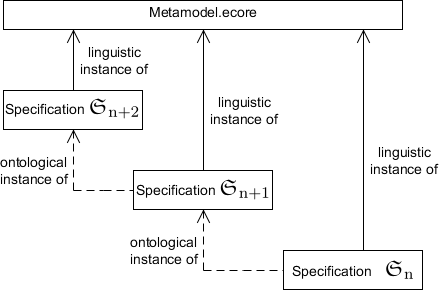
\includegraphics[scale=0.7]{./Figures/metamodelSpecification_1.png}
	\caption[Specification relationship with core meta-model]
	{Relationship between layers of DPF specifications.}
	\label{fig:core_metamodel}
\end{figure}

The ``Metamodel.ecore'' represents the linguistic meta-model that DPF provides
to describe the language syntax for every single specification created by the DPF
Model Editor.
However, other than consisting of an underlying graph and a set of constraints,
a DPF specification $\spec{S}$\textsubscript{n} is also an instance of another
specification$\spec{S}$\textsubscript{n+1}, and this is where it gets
challenging. We can describe these specification models as
ontological meta-models, since these models describes a domain specific modeling
language through an arbitrary hierarchy of models. We have to find
a way around this for our solution, because model transformation environments
that utilize Ecore based models does not allow Ecore instance models to represent
abstract syntax. This could serve a potential problem when integrating a model
transformation environment with DPF. Modeling elements that DPF provides are
created as nodes and arrows from an Ecore based meta-model, but are at the same
time created according to modeling elements one abstraction layer higher.

We will discuss how we address and approach these problems in the next
chapter. But first we will look at some related work on model transformations.
We have considered the tools, The Attributed Graph Grammar
System\cite{Taentzer2004} (AGG) and Henshin\cite{Henshin_2010} that provides a
graph based approach to model transformation. We have also worked with ATLAS
Transformation Language\cite{ATL_USERMAN} (ATL), that provides a mixture of
model transformation techniques and is therefore often referred to as a hybrid
approach to model transformation. By analysing these three tools we want to
find a model transformation environment that is best suited to be integrated
with the DPF Workbench.

\section{Three different model transformation environments}
\label{tools}

These model transformation tools use different approaches to how model
transformations are applied. We have looked at tools that implement classical
rewriting steps that utilizes the theory behind graph transformations and a tool
that employs a hybrid approach to model transformations. For this survey we have
tackled a specific exogenous model transformation example that translates an
instance model of UML's activity diagram to an instance model of a Petri
Nets\cite{jensen2007coloured} model. The next two figures provides the abstract
syntax of the two corresponding languages. These figures are represented as
Ecore models, that is EMF's interpretation of OMG's MOF. It is convenient to
represent these meta-models as Ecore models since both Henshin and ATL specify
transformation rules according to such models. 

\begin{figure}[H]
	\centering
	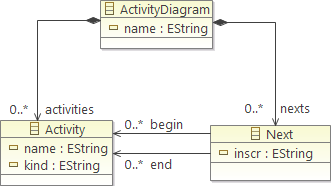
\includegraphics[scale=0.7]{./Figures/ActivityMetamodel.png}
	\caption[Abstract syntax of the source model]
	{Abstract syntax that describes the source model.}
	\label{fig:activity_metamodel}
\end{figure}

Figure~\ref{fig:activity_metamodel} represents a simplified version of a
modeling language that is provided by the general purpose modeling language UML.
The abstract syntax for the source model has an arbitrary number of activities
and next modeling elements. An activity element can have a name and a kind while
a next element can have an inscription and can either begin or end activities. The
collection of activities and next elements are provided by a specific activity
diagram.

\begin{figure}[H]
	\centering
	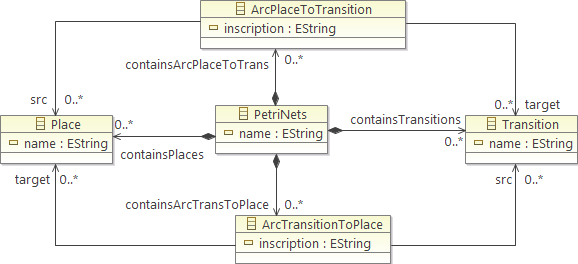
\includegraphics[scale=0.7]{./Figures/PetriNetsMetamodel.png}
	\caption[Abstract syntax of the target model]
	{Abstract syntax that describes the target model.}
	\label{fig:petrinet_metamodel}
\end{figure}

The abstract syntax for the target model consist of places and transitions. A
Petri net instance must have a place connected to a transition or the other way
around, but a Petri net model can never have two of the same modeling types
connected. For this test case we defined two nodes that specify if a connection
is between a place and a transition or a transition and a place. 

Note that these two meta-models are a simplified version of the abstract syntax
for the corresponding modeling languages. For this test case we are more
concerned with how the different model transformation environments refers to and utilizes the
abstract syntax for defining transformation rules. For each tool regardless if
the editor provides a graphical or textual syntax we discuss how to edit transformation
rules, which is relevant for how we want to design a transformation tool for
the DPF Workbench. We then consider how the different tools defines the
abstract syntax for both the source and target model. Next we specify how
transformation rules are created and if the tool provides any application
control for these rules. We finish up by mentioning how the different tools
applies a set ot transformation rules. In section~\ref{tool_choice} we consider
the model transformation environment that provides a viable model transformation
technology that could be integrated within the DPF Workbench.

\subsection{The Attributed Graph Grammar System}

AGG is a general development environment for algebraic graph
transformation systems that provides a graphical editor for creating
and modifying graphs. The editor provides a graphical user-interface with
several visual editors for applying the principles of graph transformations. AGG
also provide an interpreter and a set of validation tools. The system is an
ongoing research activity of the graph grammar group at the Technical University
Berlin and started in 1997.

\subsubsection*{Graphical Editor}
The graphical editor of AGG, represented in figure~\ref{fig:AGGScreen}, has
several functions to help the user to define model transformations. In the top
left corner of the graphical user-interface is a tree based editor that provides
a set of transformation rules, type graphs, and source graphs. The source graph
represents both the source and target model in a model transformation, and the
type graph represents the abstract syntax for the modeling languages. The
source-target relationship of a source graph is one and the same, but we will
discuss this in future sections. For the purpose of this thesis we will
refer to the host graph as the source graph, since AGG call these graphs for
host graphs.

Each transformation rule has two visual editors, representing the left
(LHS) and the right hand side (RHS), also referred to as the pattern and the
replacement graph. The tree based editor also provides the possibility to attach
application conditions to transformation rules. This is convenient if the user
wants to specify constraints that restricts the pattern or replacement graph to
be applied accordingly to a specific application condition.

Type graphs are described more in depths in the next section, but basically
the type graph defines the abstract syntax for the source and the target model.
The users can now create model instances that represents the concrete syntax of
a specific modeling language. This representation of the abstract syntax are
represented in a source graph and conforms to a corresponding type graph.

The transformation rules can also be extended with Java expressions. This means
that the users can use Java primitives such as strings, integers or float numbers to
form the pattern graph or the left hand side of the rule. However, the users
can only bind attributes that are defined in a corresponding type graph.

Figure~\ref{fig:AGGScreen} also represents some node elements and association
elements. These are meta elements that are initialized in a type graph and
are used to model the source graph, the different transformation rules and the
application conditions. Note that both the node elements and association
elements in the figure has been scaled up for the purpose of this paper.

\begin{figure}[H]
  \centering
    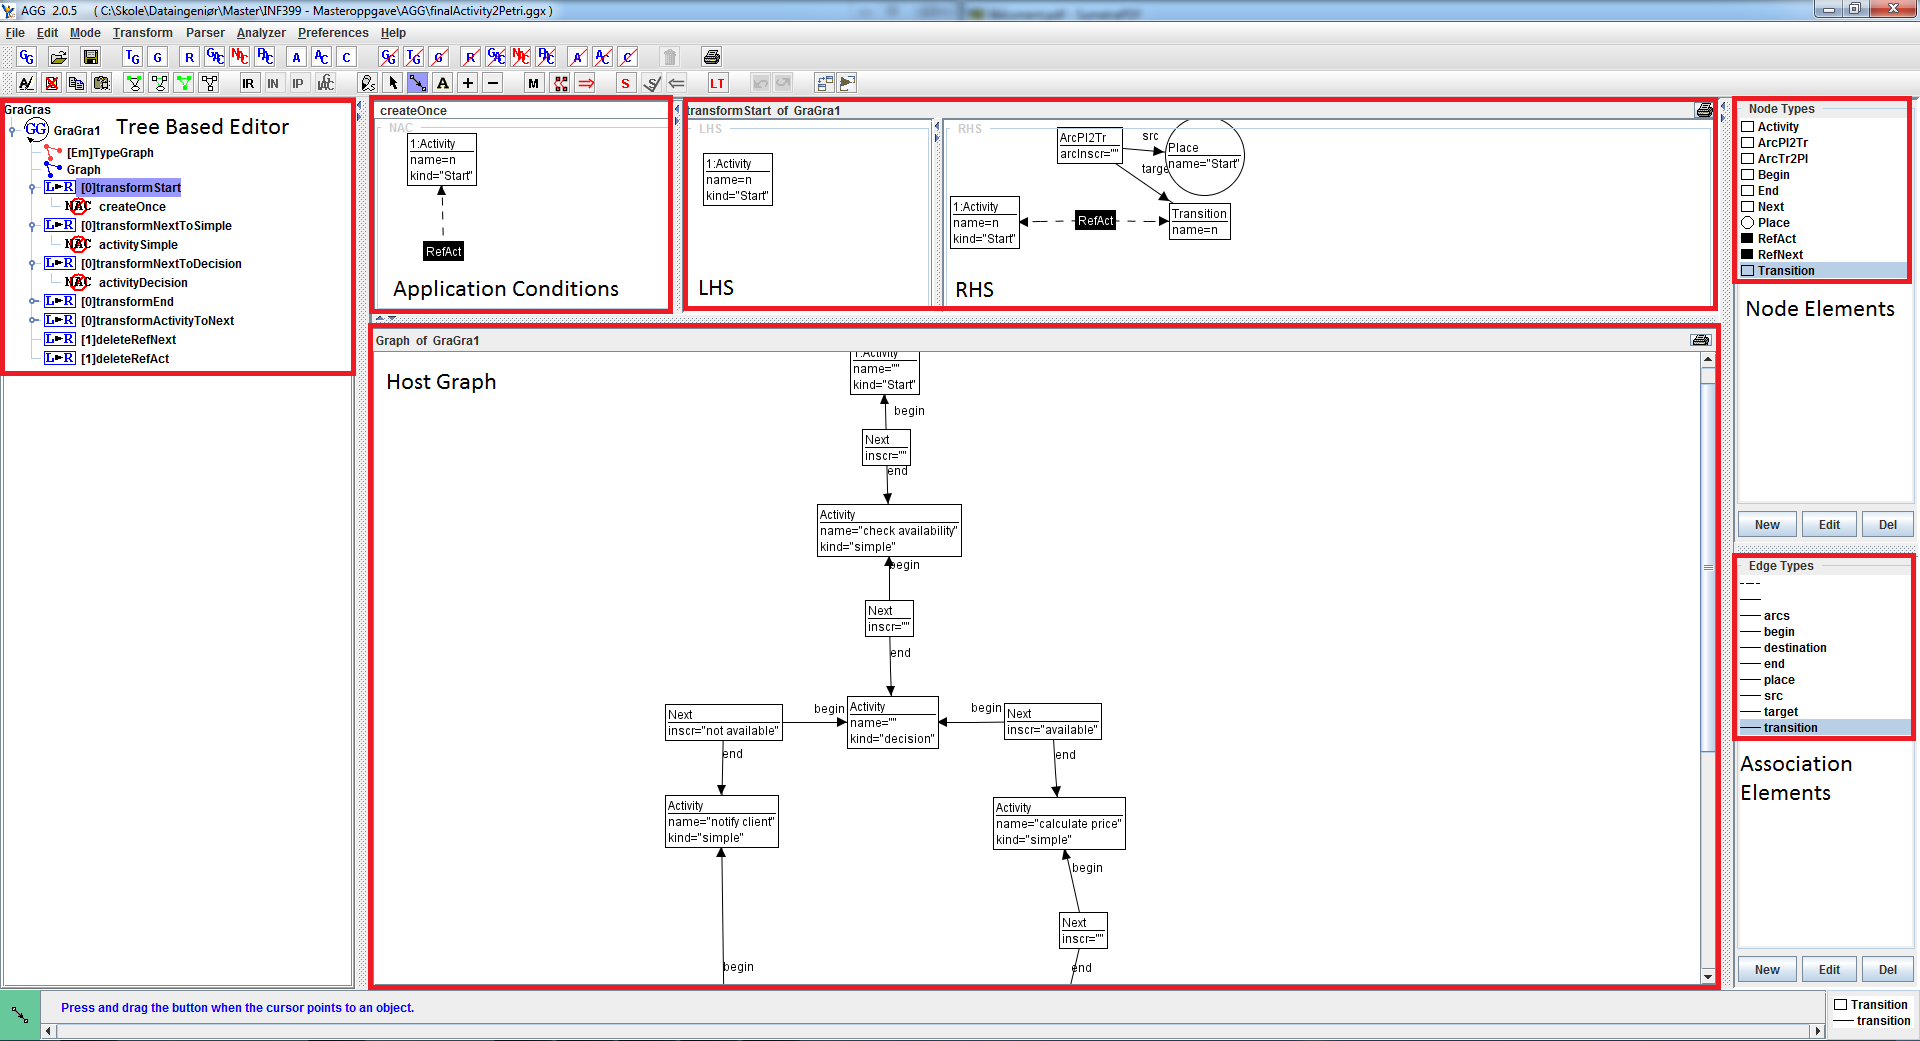
\includegraphics[scale=0.3]{figures/AGGscreen.png}
    \rule{35em}{0.5pt}
  \caption[Graphical Editor for AGG]
  {A model transformation for the AGG Editor.}
  \label{fig:AGGScreen}
\end{figure}

\subsubsection*{Defining Meta-models}

Before a source graph can be created, we have to specify the modeling
language for the source model and the target model. In AGG both the source and the
target meta-model are defined in one common type graph, that
represents the abstract syntax for both the source and target model. If we want
to prepare an AGG graph for a model transformation, we create a type graph with
references between source modeling elements and target modeling elements.
Because AGG is unaware of the relationship between these modeling elements
unless we explicitly initialize them. The relationship between source and
target modeling elements in the abstract syntax has two major purposes for an
exogenous model transformation in AGG. The relationship specifies how source
modeling elements correspond to target modeling elements and determines upon
execution of the transformation rules that a matched pattern is only applied
once.

\begin{figure}[H]
	\centering
	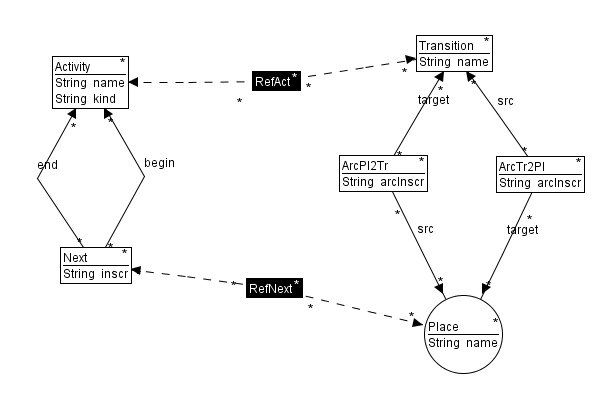
\includegraphics[scale=0.7]{figures/AggTypeGraph.png}
	\rule{35em}{0.5pt}
	\caption[Type graph in AGG]
	{Type graph for activity diagram and Petri Net in AGG.}
	\label{fig:AggTypeGraph}
\end{figure}

Figure~\ref{fig:AggTypeGraph} represents the type graph for our test case. The
abstract syntax contains nodes and arrows that include a structural multiplicity
constraint. The user defines nodes and arrows for each meta element for both
the source and target model that other than defining the abstract syntax
also defines the semantics of the two modeling languages. This is achieved by
using either the Edge Type Editor or Node Type Editor, which are editors that
defines either a node or an edge. The nodes and edges are given names and
graphical properties such as colors and a visual representation. Nodes
represents modeling elements from the two modeling languages while arrows
represents the associations between these modeling elements. In the type graph
we want to distinguish between associations and correspondences, and therefore
we represent a correspondence between a source and target modeling element as a
dashed arrow. The dashed arrow has the same properties as the association arrow
between nodes, but the graphical representation is different. This makes the
concrete syntax in the source graph easier to read when we are applying the
transformation rules. In figure~\ref{fig:AggTypeGraph} we can see that a RefAct
node is defined and is connected between the activity element and the
transition element. The same initialisation is defined between the next element
and the place element. This reference edge specifies that there is a
correspondence between Activity and Transition and between Next and
Place when the transformation rules are applied. For this type graph there is a
structural multiplicity constraint for the nodes and edges. This means that
there can be an arbitrary, or a zero to many number of instances of these nodes
and edges in the source graph and the translated target graph. 

\subsubsection*{Defining Transformation Rules}
\label{sec:AGG_rules}
Now the type graph has been initialised and the instance graph of the
source model has been created. But to be able to translate to a target model,
we need to create a set of transformation rules. A transformation rule is
initialised with an unique name, an empty LHS graph and an empty RHS graph. 

\begin{figure}[H]
	\centering
	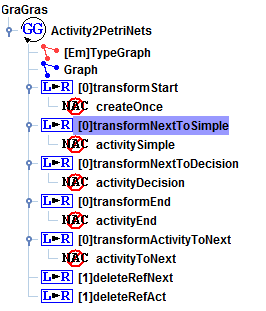
\includegraphics[scale=0.7]{figures/AGGTreeBasedEditor.png}
	\rule{35em}{0.5pt}
	\caption[Tree based editor in AGG]
	{Tree based editor for transformation rules.}
	\label{fig:AGGTreeBasedEditor}
\end{figure}

Whenever changes are made in the two graphs, AGG validates if the LHS or the RHS
conforms to the type graph. The user is unable to insert elements in the two
graphs that are not initialised in the type graph and the users are not allowed
by AGG to create associations between nodes that are not initialised in the type
graph. This is how the environment keep the source and target models consistent.
In figure~\ref{fig:AGGTreeBasedEditor} we can see the tree based editor in AGG,
that provides the type graph, the source graph and a list of transformation
rules. When a new rule is created, both the LHS and the RHS are initialised. The
users can then specify a graph structure that forms the LHS graph that AGG use
to locate matching patterns in a source graph and a RHS graph, that represents
the graph structure that the transformation system produces for each located match.
AGG provides two visual editors for these corresponding graphs. However, there
is also a graph that represents the intersection between the LHS and the RHS.


\begin{figure}[H]
	\centering
	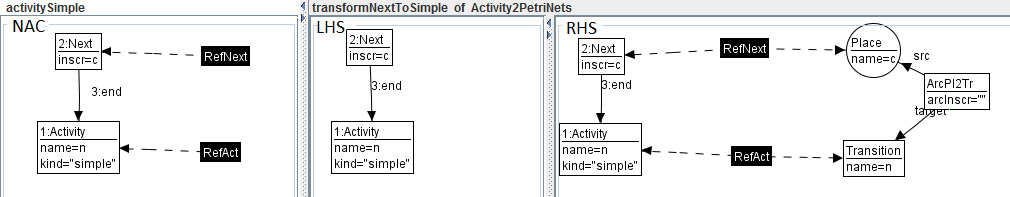
\includegraphics[scale=0.5]{figures/LHSvsRHSAGG.png}
	\rule{35em}{0.5pt}
	\caption[Representation of a rule in AGG]
	{The LHS and RHS of a rule and a NAC attached.}
	\label{fig:LHSvsRHSAGG}
\end{figure}

Figure~\ref{fig:LHSvsRHSAGG} is a representation of the rule
transformNextToSimple with the LHS and the RHS graph. The LHS contains the
graph structure that is used to locate matches while the RHS contains the
graph structure that replaces the located matching pattern. For this rule the
modeling elements that are represented in the LHS are also part of the graph
structure in the RHS graph. Modeling elements that are part of both the LHS and
RHS graph can be mapped together to specify for a transformation engine that
these modeling elements defines a graph structure that is an intersection
between the LHS and the RHS graph. In section~\ref{sec:graph_based} we
introduced the concepts of single and double pushout of graphs for graph based
model transformation tools. A double pushout of graphs includes this
intersection graph for a transformation rule that makes it possible to preserve
modeling elements that is part of both the LHS and the RHS and to make sure
that the gluing condition is valid. Modeling elements that is defined in the LHS
graph and not the RHS graph are removed when the AGG transformation engine
applies a transformation rule. For example the transformation rule in
figure~\ref{fig:LHSvsRHSAGG} locates the graph structure that the LHS defines
in a source graph and inserts a new graph structure that the RHS defines in the
source graph. This transformation rule will not remove any modeling elements
once applied since we have specified that the modeling elements in the
the LHS graph are also part of the RHS graph. A rule can also specify
application conditions that can either be a Positive Application Condition
(PAC) or a Negative Application Condition (NAC).
Figure~\ref{fig:LHSvsRHSAGG} has a NAC, activitySimple that makes sure that the
LHS of the rule is translated only once for each pattern match found in the
source graph. This is because for each applied transformation rule we preserve
the LHS graph structure and therefore is a potential match the next time the
transformation rule is applied. However, the negative application condition
requires that the matching pattern should not contain any references and
therefore is not a valid matching pattern. Through the use of these application
conditions, the users can create restrictions to how each transformation rule
should handle matching patterns in the source graph. A transformation rule
can have multiple application conditions attached.

\subsubsection*{Application Control for the Transformation Rules}

In subsection~\ref{sec:app_control} we specified that the application control of
a model transformation environment handles the match location and rule
application control. Locating matches in AGG are designed by some non-deterministic search
algorithms that the users have no specific control over. AGG does however
provide the users with the possibility to explicitly specify how the transformation rules
are applied. By default, the transformation rules are applied
non-deterministically. This means that there are no pattern to how the
transformation rules are applied and the transformation rules can be applied
differently on different runs. This option is quite useful if the set of
transformation rules are independent of each other. AGG also provides other
ways of applying rules such as applying rules by layers or by sequences. When
the scheduling mechanism is set to be applied by rule layers, then AGG introduce
the users with an integer that specify transformation rules on different layers.
This integer will range from 0 \ldots n, where the lowest number represents the
highest property.
If there are rules with the same layer number, then these rules are internally
applied non-deterministically. If the rules are applied by sequence then the rules will
be applied from the first element in the tree based editor and applying the rest
of the rules in sequence.

\subsubsection*{Translating the Source Graph}

In section~\ref{sec:AGG_rules} we described that when applying a transformation
rule a matching pattern is located in the source graph, and a graph structure
from the RHS is inserted in the same graph. This is special for AGG since
the source graph represents both the source model and the target model in a
model transformation. AGG's transformation system provides an in-place model
transformation directly on the source graph. An exogenous model transformation
that is specified in AGG usually include located matches from the source graph
in the translated graph for each transformation rule. These modeling elements that
represents the abstract syntax of the source model can then be removed through
a set of transformation rules after the modeling elements that correspond to
the abstract syntax of the target model is translated. This means that for an
exogenous model transformation we should be careful when applying the
transformation rules non-deterministically to avoid losing data. The user can
now either press Start Transformation or perform the transformation one step at
the time. For the first option AGG will apply one rule at the time until there are no more matching
patterns located in the source graph. When AGG cannot find any more matches,
the input graph is either correctly translated or there are errors in the rules.
The other option gives the user the same result as the first option, but now the
user can do one match at the time for each rule. AGG utilize both the single
and double pushout approach when executing transformation
rules\cite{Taentzer2004}. Like we discussed in section~\ref{sec:graph_based} the
single pushout approach removes the graph structure from the LHS and inserts
the graph structure from the RHS in the source graph. If the rules specifies an
intersection graph between the LHS and RHS graph then the double pushout
technique is applied. AGG's transformation engine interpret a transformation
rule and applies the transformation rule accordingly. Another model
transformation environment that utilizes the concepts of graph transformations
is Henshin.

\subsection{The Henshin Project}

The Henshin project\cite{Henshin} provides a transformation
language and a tool environment for defining model transformations for the
Eclipse Modeling Framework. The Henshin project is part of the Eclipse Model
Framework Technology (EMFT), that acts as an EMF subproject for new
technologies that extend and utilize EMF. The Henshin Editor was initially
developed in a student project at Technical University of Berlin in 2010, and
extended in the bachelor thesis \cite{JohannSchmidt} published by Johann Schmidt
and the master thesis \cite{AngelineWarning} published by Angeline Warning.
The Henshin project provides a transformation language based on graph
transformations that supports both endogenous and exogenous model
transformations. With the help of a graphical editor, Henshin provides the user
with an intuitive approach to defining transformation rules. The Henshin tool
environment also provides a transformation engine and a state space generator.

\subsubsection*{Graphical Editor}
Henshin model transformation environment is integrated as a plugin for the
Eclipse Integrated Development Environment\cite{Eclipse} and provides a
graphical editor to create and modify transformation rules. 

The users start out with using the Eclipse wizard to create an empty Henshin
document. The Henshin document is based on the commonly known Extensible Markup
Language (XML)\cite{XML}. If applicable a Henshin diagram file can be created
based on the Henshin file that gives the users an intuitive approach to
creating transformation rules.

The Henshin transformation file is represented in a tree based editor called
the Henshin Model Editor. Figure~\ref{fig:Henshin_TreeEditor} represents the
editor that contains a list of transformation rules. These transformation rules
are included under a Module element that represents the root element for a
Henshin model transformation. For this specific example there are two external
Ecore models included in the editor, more specifically the source and target
meta-models. These meta-models are created based on the EMF standard for
creating models and are independent of each other. Please note that a Henshin
model transformation can include 0 \ldots n models and therefore is not
restricted to have exact one source and one target meta-model.

\begin{figure}[H]
	\centering
	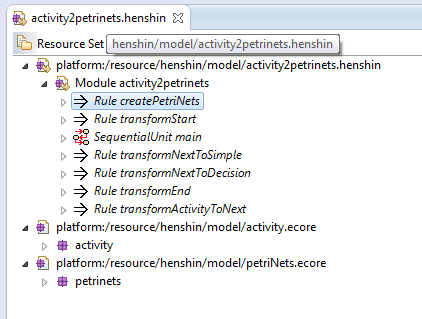
\includegraphics[scale=0.7]{figures/Henshin_TreeEdtiro.png}
	\rule{35em}{0.5pt}
	\caption[The Henshin Model Editor]
	{Tree Based Editor for rules in Henshin.}
	\label{fig:Henshin_TreeEditor}
\end{figure}

\subsubsection*{Defining Meta-models}
\label{sec:henshin_metamodeling}

The Henshin language requires a source and a target meta-model to be able to
perform model transformations. The target meta-model can either be the same as
the source meta-model or defined in another modeling language. Either way, before
the users can start creating transformation rules, the meta-models has
to be defined. To define these meta-models Henshin utilizes Ecore that is
provided by the Eclipse Modeling Framework\cite{Steinberg2009}. Ecore models
can either be created using a tree based editor called Sample Ecore Model
Editor or by using a graphical editor. While the graphical editor is optional,
the tree based editor is mandatory for creating Ecore models.

Initially the user has to create an EPackage element in the newly created Ecore
model. Henshin interpret instances of this EPackage as EObjects and is what
Henshin searches for when the user want to import an Ecore model. This EPackage
element can have several child elements, like for example EClass, EEnum and
EData type, but for this specific example we only needed the EClass
modeling element. For each EClass modeling element the users can specify an
EReference that connects two EClass modeling elements. This means that an
EReference element defines relations between the nodes for the meta-models. To give an
EClass element properties, the user can create an EAttribute element.
This element can be typed, either by a predefined list of types or by defining
user created EData types. For the purpose of this case study we only needed to
name the different nodes and therefore we only needed the data type EString.
Through the use of these Ecore modeling elements we can create the two
meta-models from figure~\ref{fig:activity_metamodel} and
figure~\ref{fig:petrinet_metamodel} that was previously presented in this
chapter.


\subsubsection*{Defining Transformation Rules}

Now we have defined the source and target meta-model for a Henshin module. We
can now use elements from the two meta-models to create transformation rules in
the Henshin transformation language. In Henshin, objects are referred to as
nodes and links between objects as edges. From the meta-models these nodes
represents the EClass elements and edges is a EReference between these EClass
elements. A collection of these nodes and edges defines a graph structure. Each
transformation rule in Henshin specifies two graphs that represent the LHS and
the RHS. Note that the graphical editor provides an integrated view to creating
transformation rules, and therefore Henshin handles assignment of modeling
elements to the LHS and the RHS through the use of stereotypes.
Figure~\ref{fig:HenshinScreen} represents a visualization of the graphical
syntax and includes a transformation rule, ``transformSimpleActivity''. On the
right side there is a tool bar that contains Henshin modeling elements and
different EPackages. The first two EPackages represents modeling elements for
the source and target meta-model. The Henshin Trace Model provides support for
including traceable links for exogenous model transformations in Henshin that
keeps track of the translated modeling elements during a model transformation.
This model consist of a single class Trace, that has two references called source
and target. These references are of type EObject and therefore can refer to any
EMF object. The Trace model is generic and therefore supports creation of
traceable links between any Ecore models.

\begin{figure}[H]
	\centering
	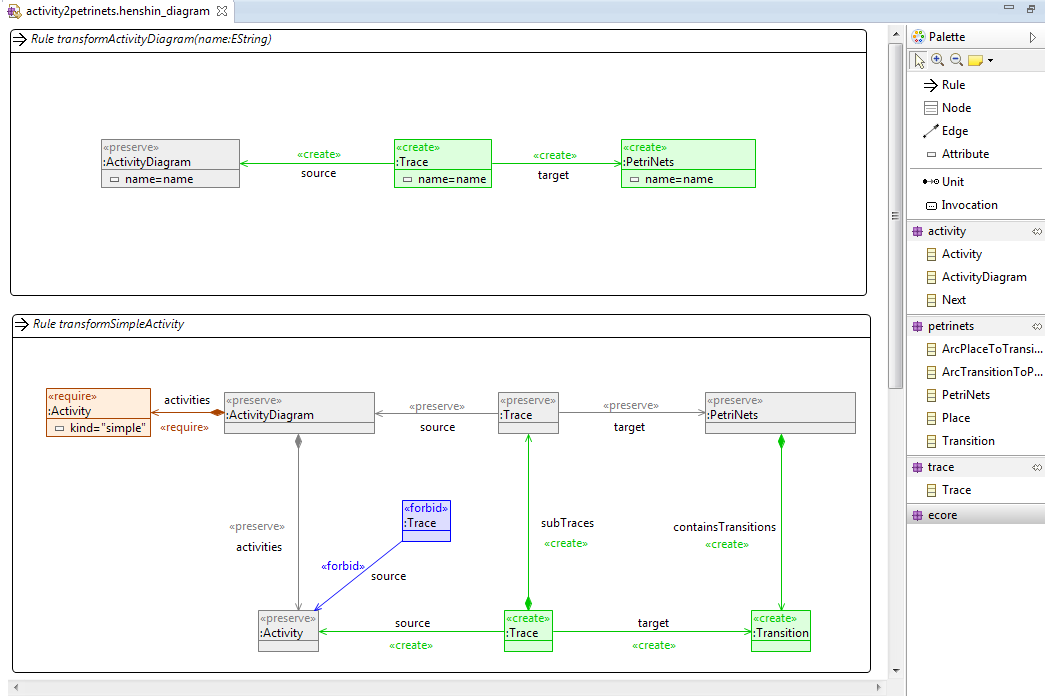
\includegraphics[scale=0.6]{figures/henshin_scren_2}
	\rule{35em}{0.5pt}
	\caption[The Henshin graphical editor]
	{A rules represented in the Henshin graphical editor.}
	\label{fig:HenshinScreen}
\end{figure}


The Node, Edge and Attribute modeling elements are used to define the different
transformation rules in Henshin. A new transformation rule in Henshin always
have to start with creation of a new Rule element. Inside this Rule element the
users are free to create nodes and define relationship between these nodes with
edges. These modeling elements are required to be created accordingly to a
corresponding meta-model.
The nodes and edges defines a graph structure that is used to either locate
matches in a source model or translate to target modeling elements. 
Note that the Node and Edge are special modeling elements for Henshin and are
used to create the content of the transformation rules. The Node element has a
type that correspond to an EClass while the Edge element has a type that
correspond to an EReference. The Ecore models that are represented in
figure~\ref{fig:HenshinScreen} has a list of modeling elements that are typed
by EClass. These modeling elements are a shortcut for Henshin that creates a
Henshin node with a corresponding EClass type. The Attribute element can be used
if attributes are defined for the classes that are imported. We will come back to
the Unit element in the next section. Henshin distinguish if nodes, edges or
attributes are part of the LHS and the RHS through the use of predefined
stereotypes, or action types. Based on these action types Henshin automatically
specifies if these modeling elements defines a graph structure that is used to
locate matches in a source model or produce modeling elements for a target
model. If the action type consist of the sequence ``create'', Henshin knows
that this element should be part of the replacement graph, or the RHS. While on
the other side, the sequence ``delete'' should be part of the pattern graph, or
the LHS. The ``preserve'' sequence is a bit more special, because nodes or
edges in Henshin that is specified by this action type should be part of both
the LHS graph and the RHS graph. This is done by putting the preserve element
in both graphs and then create a mapping between these two elements to inform
the Henshin Interpreter that this represents the same element. Henshin also has
support for application conditions through the action types ``forbid'' and
``require'', that are used for defining Negative Application Conditions (NACs)
and Positive Application Conditions (PACs). These actions are supported for
nodes, edges and attributes. The example rule in figure~\ref{fig:HenshinScreen}
use four of these action types. The modeling elements in gray represents
modeling elements that are part of both the RHS and the LHS graph, while the
modeling elements in green are specified in the RHS graph. This specific
transformation rule will locate a matching pattern in a source model that is
described by an Activity modeling element. The positive application condition
specifies that Henshin only should locate matches that is of kind ``simple''.
The negative application condition specifies that a located match that is
described by the Activity class should not have a traceable link.
The NAC specifies that the transformation engine does not locate duplicate
matching patterns. The first time a match is located a traceable link is
established. Now this specific match is no longer a valid match since the NAC
forbids the transformation engine to locate matches that already has
established a traceable link to this modeling element. Note that we have a
Trace and a PetriNets that is both a preserve modeling element. This is because
these two are already translated by an already applied transformation rule. The
transformation engine provides in-place transformations for exogenous model
transformations and an already applied transformation rule has translated the
Trace and PetriNets modeling element and are now part of the source model. The
transformation engine can now include these translated target modeling elements
in search patterns for other transformation rules. 

\subsubsection*{Application Control for the Transformation Rules}
Transformation units are used to administrate the different transformation
rules. Henshin provides several different units with different properties.
Note that a transformation rule is also a transformation unit. This means that
it is unnecessary to create an unit in Henshin if a model transformation only
consist of a single transformation rule. However, if there are more than one 
transformation rule there has to be a control mechanism that determines how
these transformation rules should be applied. An Independent Unit applies
rules non-deterministically, which is a good solution if the order of applying
the transformation rules is not important and the rules are independent of each
other. But if the transformation rules requires a very strict pattern and are
dependent of other rules, then a sequential unit are a safe way to apply rules.
The sequential unit forces the Henshin transformation engine to apply rules in
a sequenital order. Figure~\ref{fig:SequentialUnitHenshin} is an example of a
sequential unit that will start applying rules at the black circle and follow
the arrow through each given rule until it is finished.  

\begin{figure}[H]
	\centering
	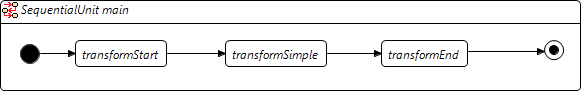
\includegraphics[scale=0.7]{figures/SequentialUnitHenshin_1.png}
	\rule{35em}{0.5pt}
	\caption[A Sequential Unit in Henshin]
	{A SequentialUnit main that contains a sequence of rules.}
	\label{fig:SequentialUnitHenshin}
\end{figure}

If applicable a transformation unit can also consist of other units, for example
if the user want to either iterate or loop through a transformation rule. The
previous section described an example of a rule in
figure~\ref{fig:HenshinScreen}. The sequential unit in
figure~\ref{fig:SequentialUnitHenshin} includes a LoopUnit
``transformSimple'' while the ``transformStart'' and ``transformEnd'' represents a
single rule. The loop unit applies a single transformation rule until there are
no more matches found in a source model.
This is convenient for the rule, ``transformSimpleActivity'' since we specified
that the rule should only locate matches where there exist no traceable link.
Henshin also has two other units that can administrate transformation rules,
namely ConditionalUnit and PriorityUnit. The ConditionalUnit follows an if-else
pattern, and is used if the user want Henshin to choose between two units.

\subsubsection*{Translating the instance model}

Now that we have defined the source and target meta-model, created a set of
transformation rules and initialised a control mechanism for these rules it is
time to apply the transformation rules. For Henshin there is two ways to do
this. In Henshin the default engine for executing model transformation is the
Henshin interpreter. This interpreter can be invoked either by using the an
Eclipse wizard or programmatically using the Henshin API. 

Using the Eclipse wizard is done by opening the Henshin file in the Henshin
Model Editor and right clicking the root object and apply transformation.
This will open a wizard where the user can choose a transformation unit, which
will either be a single transformation rule or some transformation unit that
applies other units or rules. The user also has to select the instance
model and can explicitly set parameters for the rules if this is applicable.
Now the user has two choices, the first choice is to preview the result of the
model transformation. This will either show the user a new window with the
modifications to the model or a message that the rule or unit could not be
applied. If the user press Transform instead of Preview, the model will be
transformed and saved.

The interpreter can also be invoked programmatically, either as an
Eclipse based application or as a simple Java application. Henshin provides an
API that lets the users invoke the interpreter through the use of Java code and
use the strengths of Henshin in their own program. There is a class
HenshinResourceSet that lets the user load and save models and
load a Henshin model transformation. When the instance model and Henshin module
is loaded into the resource set, the transformation can be applied through the
use of the Henshin Engine class. This is where Henshin finds and translates
matches found in the instance graph. The user also has to specify the main
transformation unit from the Henshin module. Both the engine and the unit can be
loaded into the UnitApplication class. This class has a method that lets the
user execute the model transformation. If the transformation was executed
without errors, then the instance model can be saved with the translated
changes.

\subsection{ATL Transformation Language}

ATL\cite{Jouault2008} (ATL Transformation Language) provides a model transformation
language and is an implementation of the QVT\cite{QVT} standard. It
provides ways to produce a set of target models from a set of source models.
ATL is maintained by OBEO\cite{OBEO} and AtlanMod\cite{ATLANMod} and was first
initiated by the AtlanMod team, previously called the ATLAS Group, located at
the University of Nantes in France. The initial version of ATL was created in
2004, where ATL later became part of the Eclipse Generative Modeling
Technologies (GMT) \cite{GMT}. The goal of GMT is to produce a set of research tools in the
area of Model Driven Software Development. The ATL Integrated Development
Environment (IDE) was later promoted for the Eclipse M2M project in January
2007.

There are developed several tools that has support for a declarative
approach to model transformation. ATL is a hybrid model transformation
approach, which is a transformation language that combines other model to model
transformation approaches. For example, ATL provides transformation rules that
can be either fully declarative or fully imperative or a mixture of both. 

\begin{figure}[H]
	\centering
	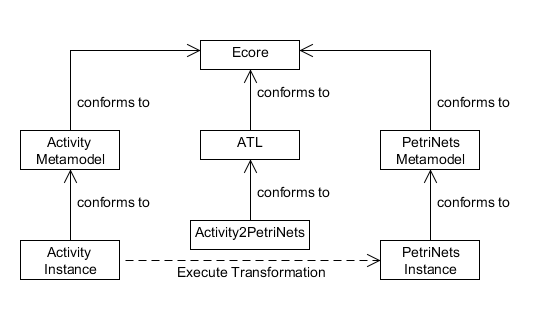
\includegraphics[scale=0.55]{figures/ATL.png}
	\rule{35em}{0.5pt}
	\caption[Model transformation for Atlas transformation language]
	{Model transformation process for Activity2PetriNets.}
	\label{fig:ATL}
\end{figure}

Figure~\ref{fig:ATL} gives us an idea of how the ATL transformation from an activity
diagram to Petri net are handled. We want to generate an instance model of
PetriNets that conforms to its own meta-model. This is generated from a source
model, Activity Instance that conforms to its respective meta-model.
The created transformation Activity2PetriNets is expressed in the ATL
transformation  language, that conforms to its own meta-model. These three
meta-models conform to the meta-model Ecore. So this makes Ecore a metameta-model
to represent the meta-models of Activity, ATL and PetriNets.

ATL has to be configured properly before the user can execute a model
transformation. In this configuration both the location of the source and target
meta-model requires to be implicitly specified. The user also has to specify
the instance model that should be translated, and create a new file that can be
specified as the target instance model for the ATL run configuration. The user
can then initiate the transformation by running this as an ATL transformation.


\subsubsection*{Textual editor}

ATL can be compared to a programming language, because it
basically is a transformation language that provides a concrete textual syntax.
ATL is a text based transformation language, and is build around the Object
Constraint Language (OCL) \cite{OCL} with some additional predefined functions.
ATL transformations is stored in a file extension called \textit{``.atl''.}
These ATL files can contain different kind of ATL units and are defined in its own
distinct ATL file. These different ATL units are ATL modules, ATL queries and
ATL libraries. Libraries can be used to create independent ATL libraries that
can be imported and used in different ATL units. The module unit
specifies the different application rules for a  model transformation and
queries are used when the users want to compute primitive values from the
source models.

Now that we have specified these three ATL units, we can shortly describe how
we can use the ATL transformation language to create model to model
transformations. For our case study, we only need the ATL modules. This unit
enables developers to specify a set of rules that produces a set of target
models from a set of source models. The source and target models of an ATL
module must be consistent with their corresponding meta-models. 

\subsubsection*{Defining Meta-models}

Defining meta-models for the ATL language is defined by the modeling language
Ecore. Since the meta-models are defined similar to Henshin, see
section~\ref{sec:henshin_metamodeling} for more details. 

At first, the user start out with a blank ATL file. Since we are working in
the ATL Integrated Development Environment for Eclipse, we want to start the
document with defining the path to the source and the target meta-model. The
reason for doing this is to achieve auto completion for modeling elements
defined in the Ecore meta-models, which is convenient for the users when
creating transformation rules.  

\begin{figure}[H]
	\centering
	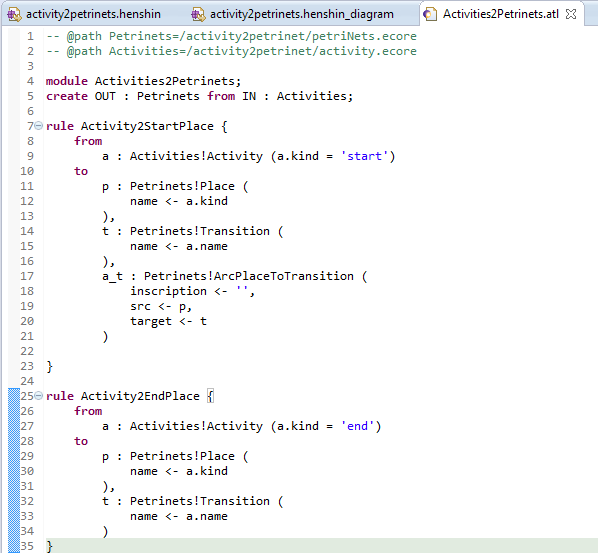
\includegraphics[scale=0.5]{figures/ATLScreen.png}
	\caption[Simple rules for ATL]
	{Two simple rules for Activity2PetriNets in ATL.}
	\label{fig:ATL_Screen}
\end{figure}

Next the file is composed of a header section, where the user can give the
module a name and specify the source and target meta-models. Note that the
module name has to be identical to the name of the ATL file for the
transformation engine to be able to extract the information.

We also need to specify the source and the target meta-model. From
figure~\ref{fig:ATL_Screen} we can see that the target meta-model is initialised 
with the keyword create, and the source meta-model is initialised using the
keyword from. The user can also import some existing libraries if needed. This
import section is however optional. Importing meta-models are handled a bit
differently in ATL compared to Henshin. In ATL the meta-models are imported
explicitly while in Henhsin they are imported implicitly before they can be used
in modifying the transformation rules. For ATL the user has to configure where
both the source and the target meta-model are located through a configuration
page. 

The next element is a set of rules that defines how the target models are
generated from the source models. These rules are used to implicitly match
source modeling elements and produce target modeling elements. In
figure~\ref{fig:ATL_Screen} we have examples of two rules, namely the rule for
transforming the start activity and the rule for transforming the end activity.
We can see that for each rule we specify what we want to translate from and
what we want to translate to. We will describe transformation rules in more
details in the next section.

The last element in a ATL module is a set of helper functions. This collection
of helpers can be compared to Java methods and can be used to make the
transformation rules easier to read.

\subsubsection*{Transformation Rules}

A rule in ATL describes how a target model should be generated from a source
model. In ATL there are three different types of rules, the matched rules and
the lazy rules are both fully declarative while the called rules are imperative.
These rules have an input pattern and an output pattern that consist of
variables that specifies the different source and target modeling elements. The
input pattern can have a list of source modeling elements that is part of a
rule by defining a new variable for each different modeling element. Each input
pattern element requires a mandatory type that corresponds to a meta-class
defined in a corresponding meta-model. The output pattern defines how the target
model elements are created from the input model.

\textbf{The matched rules} provides an declarative approach to
creating transformation rules in ATL. The users can specify from which kinds of
source modeling elements the target modeling elements can be generated from and
how the generated target modeling elements should be initialized. A matched rule
locates a match according to the type of the source modeling elements and generate target modeling
elements from these matches. A new matched rule is defined by the keyword
``rule'' and has two mandatory and two optional sections. The mandatory
sections specifies the input pattern and the output pattern while in the first
optional section the users can declare and initialize local variables. Note
that these variables can only be used within the scope of a rule. The second
optional section includes an imperative section if the users want to specify the
behaviour of a rule. The type that is introduced in the input pattern
conforms to a meta-element in a meta-model of the source model. This rule will
then generate target elements according to each match in the source model.

Figure~\ref{fig:ATL_Example} shows a simple rule, Activity2StartPlace that
translates Activity source elements to some target elements. This rule
specifies the keyword \textit{from} for the input pattern and \textit{to} for
the output pattern. For this example we want to find matches for one source
element that is of type Activity that conforms to the meta-model Activities. We
also provide additional properties for this input source element, where we only
want to find matches that conforms to the type Activity and has the name
``start''. The rule specifies that we want to generate three target pattern
elements p, t and a\textunderscore t from this matching type. These generated
target elements conforms to the meta-model Petrinets and specifies that these
generated types should generate attributes from the source pattern element. The
generated target model elements is initialized with attributes from the matched
source pattern element.

\begin{figure}[H]
	\centering
	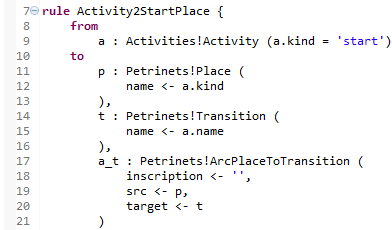
\includegraphics[scale=0.7]{figures/ATL_Example.png}
	\caption[Example of a matched rule in ATL]
	{An example of a matched rule in ATL.}
	\label{fig:ATL_Example}
\end{figure}

If applicable the users can add an optional condition for each rule to check for
certain matches for this input element. This condition is expressed as an OCL
expression and gives the user the possibility to restrict the searches of the
source elements. 

The second type for ATL rules are \textbf{Lazy rules}. These lazy rules will
never be applied when a model transformation in the Atlas Transformation
Language is executed unless they are applied at runtime by either a matched or
a called rule. These lazy rules are created similar to the matched rules.

The third and final type for ATL rules are \textbf{Called rules}. A
called rule has to be called from an imperative section from a rule.
A called rule is created similar to a matched rule, namely with a \textit{rule}
keyword. One thing that is special with a called rule is that it does not have
to match source elements from the source model. A called rule can for example
include an imperative section for a matched or lazy rule that defines the
semantics of the rule.

\subsubsection*{Execution of an ATL transformation}

Figure~\ref{fig:ATL_Execution} describes the architecture of the transformation
language. From the figure we can see that we have an association between EMF and
Ecore models. This are the meta-models that are expressed using EMF's Ecore
model. These meta-models are then translated through a model handler that
compiles these Ecore models to the ATL Virtual Machine, where these meta-models
can be used both in creating ATL programs and in ATL's internal interpreter. The
ATL compiler translates the ATL file into a new ASM assembler file that ATL can
use to launch a model transformation. This assembler file contains the
compiled code of the corresponding ATL file.

\begin{figure}[H]
	\centering
	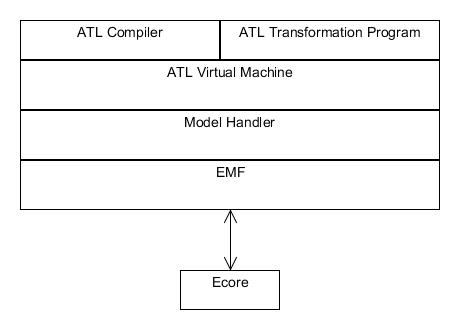
\includegraphics[scale=0.6]{figures/ATL_Execution.png}
	\caption[Internal infrastructure for ATL]
	{Internal infrastructure of for ATL.}
	\label{fig:ATL_Execution}
\end{figure}

The default semantics for executing a set of transformation rules specified in
ATL can be described in three phases. Consider ATL User Manual\cite{ATL_USERMAN}
for more detailed information.

The first phase is an initialization phase. This phase consist of amongst other
things to initialize the trace model and the module of an ATL transformation.
The trace model in ATL has one important function, and that is to create a
trace link that points to the matched source input elements and the
corresponding generated target output elements. The traceable model in ATL works
as an implicit tracing mechanism that specifies relationships between the source
modeling elements and its corresponding target modeling elements by using a
native type called ASMTransientLink\cite{Wagelaar}. For every time a transformation rule is
matched to a source element, one ASMTransientLink is created that includes the
name of the rule, a source modeling element and a target modeling element.
These links are added to a collection that is stored internally for ATL. This
means that the users of ATL cannot access these links after a model
transformation has finished executing. However, as shown by Andr\'{e}s Yie and
Dennis Wagelaar\cite{Wagelaar}, that gaining access to these ATL traces can be
done explicitly by creating transformation rules that generates a tracing model
based on the internal tracing information provided by ATL.

The next phase consist of finding matches in the source pattern based on the
matched rules. This is done by the ATL transformation engine that applies a
searching algorithm to locate valid matches. A match is valid
when all input pattern elements are found amongst the source modeling elements
and any OCL expression for that matched rule is valid.
The transformation engine also allocates the target model elements based on the
declared output pattern into memory. At this point the target modeling elements
are only allocated, they are later initialized in the final phase. For each
match found, there is created a traceable link that has a source link to the
matched source modeling elements and a target link to the generated target
modeling elements. The generated target elements are not given any attributes or
properties in this phase. This phase creates target modeling elements from
matches found and define traceable links that relates source and target
modeling elements.

The final phase for executing an ATL module is to initialize the target modeling
elements. At this stage each allocated target modeling element is given
attributes and features that corresponds to the matched rule. The ATL
transformation engine now use the traceable links to determine the matched
source modeling elements and the generated target modeling elements. This
operation is called resolveTemp, which returns the reference from the target
modeling elements that where generated in the second phase to the corresponding
source modeling element. Now that these three phases is finished the ATL
transformation engine can execute the imperative code sections defined for the
module and successfully finish a model transformation.

\section{Model transformation environment for DPF}
\label{tool_choice}

After working with the three model transformation environments in the previous
section we decided go for a solution to integrate Henshin with the DPF
Workbench.
In this section we will describe why Henshin is best suited to be integrated
with DPF. In this section we will describe why Henshin is the better choice of
the three considered environments to be integrated with DPF.
Henshin\cite{Henshin_2010,Henshin} is a relatively new installment in the world
of model transformations. Henshin was initially created three years
ago, in 2010 and is marked as an Eclipse Incubation project. The purpose of the
incubation phase is to establish a fully functional Eclipse plugin. In
theory an integration of Henshin with DPF should be possible, since Henshin
applies model transformations based on Ecore models and DPF specifications are
basically represented as Ecore models. This presents a problem with integrating
AGG with DPF since AGG does not employ Ecore modelsS. In EMF the root of all
modeling objects is an EObject that has no references to a Java Object.
AGG could be integrated with DPF, but the problem is that this would
require an extensive amount of manual coding. We could use AGG as a general
purpose graph transformation engine in a java application. We would have to
create the source model as an AGG graph and a type graph based on the source and
target modeling formalism that DPF provides. AGG provides an API that
conveniently let us create type graphs, source graphs, transformation rules and
application conditions.
 
\begin{figure}[H]
	\centering
	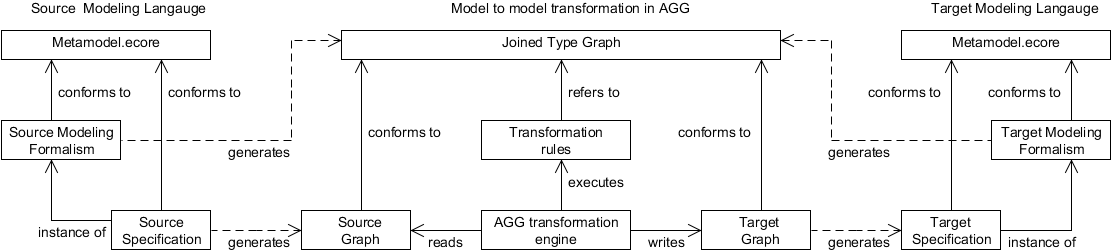
\includegraphics[scale=0.52]{figures/AGG_solution.png}
	\caption[Proposed solution for integration of AGG]
	{Proposed solution for integration of AGG with the DPF Workbench.}
	\label{fig:AGG_Solution}
\end{figure}

Figure~\ref{fig:AGG_Solution} represents a proposed solution for how to
integrate AGG together with the DPF workbench. The figure represents a
source modeling formalism on the left side, a target modeling formalism on the
right side and a model to model transformation done with AGG in the middle. The
figure illustrates that we have to generate four models to be able employ AGG
for a model to model transformation in DPF. First we create the abstract syntax
for AGG source graphs by generating a joined type graph from a source modeling
formalism and target modeling formalism. Then we have to generate the source
specification into a source graph that at the same time conforms to the joined
type graph. Note that we do not mention the transformation rules since we have
to generate these regardless of what model transformation environment we
integrate with the DPF Workbench.
After the AGG transformation engine has executed the transformation rules we
have to generate a target specification based on the translated target graph.
This leads to some potential problems. The program that generates a source graph and
a target specification has to be solid and not contain any flaws or bugs.
Another problem is to keep the models consistent throughout the model transformation.
How can we be certain that the target graph is consistent with the target
specification? It is easy to lose consistency when changing a model manually
from a target graph to a target specification. We could use AGG to do this, but
that leads to many potentially factors that could go wrong. For both Henshin and
ATL we are not required to do anything extra with these models. Since both
environments has support for including Ecore models as meta-models and requires
an instance model of an Ecore model as a input model to apply a model
transformation. Therefore AGG can be integrated with EMF with some additional
work, but Henshin and ATL is a more viable choice for DPF, since we can use
the ``Metamodel.ecore'' as a meta-model and a source specification as input
model directly in the other two environments. 

Now we need to decide if we want to try and integrate the hybrid model
transformation environment, ATL or the graph based model transformation
environment, Henshin. In section~\ref{sec:DPF} we discussed that a DPF
specification is an extension of the Generalised Sketches formalism that is
basically a directed graph. A model transformation in Henshin is based on the concepts of graph
transformations and category theory. We can then be certain that Henshin can
interpret a source specification as a directed graph. Henshin transformation
language is also based on the two graph transformation styles single (SPO) and
double pushout (DPO) that we discussed in section~\ref{sec:graph_based}. And we
recall that the DPO approach provides a dangling condition that ensures that a
model transformation does not result in any edges that are missing a source or
a target node. We want to create a tool for the DPF Workbench that provides the
following.

\begin{itemize}

\item \textit{Concrete Graphical Syntax}. We want to be able to create
transformation rules based on the graphical syntax that the DPF Model Editor
provides.

\item \textit{Generic}. We want our tool to work for an arbitrary source and
target modeling formalism regardless of abstraction layer. 

\end{itemize}

The tool is required to create a set of transformation rules based on some
model transformation language and we want these transformation rules to be
generic. This means that we create a set of transformation rules based on an
arbitrary source and target meta-model. The only aspect of these meta-models
that is consistent is that they contain a list of nodes and arrows. This means
that regardless of abstraction layer a specification is specified by a set of
nodes and arrows. The reason for why we decided to integrate Henshin
within the DPF workbench is provided in the three following points. 

\begin{enumerate}

\item We want to create a tool that use a simplified version of the DPF Editor
to create transformation rules that provides a concrete graphical syntax. DPF
models are already based on category theory and provides a graphical syntax. 

\item Through the use of the Henshin meta-model we can generate a set of
transformation rules that are based on the abstract syntax of the source and
target specification. We can define a set of transformation rules in Henshin
as a java application with the help of the API that Henshin provides. 

\item We can utilize the concepts around graph transformation that provides a
left hand side, a right hand side and an intersection graph. Through these three
graphs we can in Henshin use the single or double pushout approach when applying
a set of transformation rules. 

\end{enumerate}

The problem with integrating Henshin with DPF is that Henshin is based on the
EMF technology, and therefore utilize OMG's MOF. Henshin supports out of the
box model transformation that translate instance models that conforms to an
Ecore based meta-model. These instance models provides the concrete syntax of a
modeling language and are described by a corresponding meta-model that
represents the abstract syntax. This meta-model is provided accordingly to the
second layer of the Meta-Object Facility. This means that Henshin provides model
transformation according to EMF's two layered modeling environment. DPF on the
other hand provides initialisation of a potential endless hierarchy of
meta-modeling, and therefore does not match the steps MOF provides to create
the abstract syntax for a Domain Specific Language. We know that a
transformation rule in Henshin requires references to meta-modeling elements
from a source meta-model and a target meta-model. What makes a DPF
specification special is that it is an instance model of both an Ecore based
meta-model and another DPF specification. This means that a specifications
concrete syntax is defined by the abstract syntax of a specification that is one
abstraction layer higher. In DPF we can create an arbitrary level of
meta-models and therefore two different Domain Specific Modeling Language can
be defined in different abstraction layer hierarchies. The Henshin
environment has strict guidelines on how models are imported and used. These
models are required to be created accordingly to the Ecore model provided by
EMF. Henshin can then utilize these models to create a graph pattern that
structure both the LHS and the RHS graph of a transformation rule. The LHS
graph contains a graph structure that is is used by the transformation engine
to locate matches in an instance model that conforms to a specified Ecore
model.

For our tool we can structure a set of transformation rules in Henshin based on 
this common meta-model, \textit{Metamodel.ecore} that all specifications
$\spec{S}$\textsubscript{1\ldots n} conforms to. We have to threat all
specifications similar if we want the tool to provide a generic model to model
transformation environment. The challenge with integrating Henshin in a language
workbench that provides meta-modeling at arbitrary layers of abstraction is not in the
source specification we want to translate, but in the specification
that the source specification conforms to one abstraction layer higher. This
proves to be a problem for Henshin, because we cannot import an instance model
of an Ecore based meta-model into the Henshin model transformation environment.
We can do changes to an instance model by using Henshin, but the transformation
language can only import and utilize models that conforms to the Ecore
meta-model. To solve this for DPF specifications we expand transformation rules
in Henshin with application conditions. This means that we restrict the LHS
graph to locate matching modeling elements in an instance source specification
based on the abstract syntax that another specification provides. The next
chapter provides an explanation of how we integrated Henshin for a
transformation tool that provides model to model transformations for the DPF
workbench.





%----------------------------------------------------------------------------------------
%	SECTION 2
%----------------------------------------------------------------------------------------

